
\documentclass[twoside, hidelinks]{article}


\usepackage[backend=biber,sorting=none]{biblatex}
\setlength\bibitemsep{1.5\itemsep}
\addbibresource{refbase.bib}

\usepackage{lipsum} % Package to generate dummy text throughout this template

\usepackage[sc]{mathpazo} % Use the Palatino font
\usepackage[fleqn]{amsmath}
\usepackage{lmodern}
\usepackage{pifont}
\usepackage[utf8]{inputenc} % Use 8-bit encoding that has 256 glyphs
\linespread{1.05} % Line spacing - Palatino needs more space between lines
\usepackage{microtype} % Slightly tweak font spacing for aesthetics

\usepackage[hmarginratio=1:1,top=32mm,columnsep=20pt]{geometry} % Document margins
\usepackage{multicol} % Used for the two-column layout of the document
\usepackage[small,labelfont=bf,up,textfont=it,up]{caption} % Custom captions under/above floats in tables or figures
\usepackage{booktabs} % Horizontal rules in tables
\usepackage{float} % Required for tables and figures in the multi-column environment - they need to be placed in specific locations with the [H] (e.g. \begin{table}[H])
\usepackage{hyperref} % For hyperlinks in the PDF
\usepackage{graphicx}

\usepackage{lettrine} % The lettrine is the first enlarged letter at the beginning of the text
\usepackage{paralist} % Used for the compactitem environment which makes bullet points with less space between them

\usepackage{abstract} % Allows abstract customization
\renewcommand{\abstractnamefont}{\normalfont\bfseries} % Set the "Abstract" text to bold
\renewcommand{\abstracttextfont}{\normalfont\small\itshape} % Set the abstract itself to small italic text

\usepackage{titlesec} % Allows customization of titles
\renewcommand\thesection{\Roman{section}} % Roman numerals for the sections
\renewcommand\thesubsection{\Roman{subsection}} % Roman numerals for subsections
\titleformat{\section}[block]{\large\scshape\centering}{\thesection.}{1em}{} % Change the look of the section titles
\titleformat{\subsection}[block]{\large}{\thesubsection.}{1em}{} % Change the look of the section titles

\usepackage{lipsum}

\usepackage{fancyhdr} % Headers and footers
\pagestyle{fancy} % All pages have headers and footers
\fancyhead{} % Blank out the default header
\fancyfoot{} % Blank out the default footer
\fancyhead[C]{Modelos de Reação-Difusão \ding{118} Belo Horizonte - MG, 2016} % Custom header text
\fancyfoot[RO,LE]{\thepage} % Custom footer text

\renewcommand{\figurename}{Figura}


\title{\vspace{-15mm}\fontsize{24pt}{10pt}\selectfont\textbf{Modelos de Reação-Difusão}} % Article title

\author{
    Breno M. C. C. e Souza\\
    \href{mailto:breno.ec@gmail.com}{breno.ec@gmail.com}\\
  \and
    Fernando G. D. C. Ferreira\\
    \href{mailto:fernandogdcf@gmail.com}{fernandogdcf@gmail.com}\\
}

\date{CEFET-MG} % lol


\begin{document}

\maketitle % Insert title
\thispagestyle{fancy} % All pages have headers and footers


\renewcommand{\abstractname}{Resumo}
\begin{abstract}
\noindent A taxa de atividades de materiais catalíticos sofre redução por
diversos mecanismos, sendo um deles o envenenamento de regiões catalíticas por
substâncias químicas adsorvidas, de forma que reagentes passam a não alcançar
mais tais regiões. Este trabalho trata de uma simulação cujo principal objetivo
é replicar resultados já alcançados em trabalhos prévios que, além de resultados
oriundos de simulação, também mostram resultados analíticos aproximados. O
modelo simulado trata de um sistema composto por uma rede unidimensional, com
sítios catalíticos e reagentes uniformemente distribuídos, onde tal rede é palco
de reações unimoleculares. A dinâmica do modelo se dá através da difusão dos
reagentes que possivelmente atingem um sítio catalítico, reagem instantaneamente
e deixam o sistema na forma de produto, sendo que essa reação pode desativar o
sítio catalítico com probabilidade \textit{p}. O sistema apresenta 2 fases
distintas: uma em que um número positivo finito de reagentes sobrevive à
dinâmica; outra em que há desativação de todos os sítios catalíticos da rede. A
dinâmica do sistema é regida por reação bimolecular, onde sítios catalíticos
desempenham papel da segunda espécie reativa, quando na região de fronteira
entre tais fases. O comportamento do sistema próximo da criticalidade apresenta
cruzamento, onde ele obedece lei de potência com expoente próximo de
$-1/4$ até tempos da ordem de $10^3$.
\hfill \break
\hfill \break
\textbf{Palavras-chave:} desativação catalítica, redes discretas, simulação.
\end{abstract}


\renewcommand{\abstractname}{Abstract}
\begin{abstract}
\noindent The rate of catalytic material undergoes reduction activities by various
mechanisms, one being the poisoning of catalytic regions by adsorbed chemicals,
reagents pass so that it does not reach more such regions. This work is a
simulation whose main objective It is to replicate the results already achieved
in previous jobs, in addition to results coming simulation also show approximate
analytical results. O simulated model is a system composed by a one-dimensional
network with catalytic sites and reagents evenly distributed, where such a
network is the stage unimolecular reactions. The dynamics of the model is
through the dissemination of reagents possibly reach a catalytic site, react
instantly and leave the system in the form of product, and this reaction can
disable catalytic site with probability \ textit {p}. The system has 2 phases
different: one in which a finite positive number of reagents survives dynamics;
another in which no deactivation of all the catalytic sites of the network. The
system dynamics is governed by bimolecular reaction where catalytic sites play a
role in the second reactive species, when in the border region between these
phases. The behavior near criticality system has intersection where he obeys a
power law with exponent close $-1/4$ To time in the order of $10^3$.
\hfill \break
\hfill \break
\textbf{Keywords:} catalytic deactivation, discrete networks, simulation.
\end{abstract}


\hfill \break
\hfill \break
\hfill \break
\hfill \break

\begin{multicols*}{2} % Two-column layout throughout the main article text
\newpage


\section{Introdução}

No trabalho, é realizada uma simulação de um processo de reação-difusão com
atividade catalítica a partir de modelos desenvolvidos em\cite{3}.

Esses sistemas de reação-difusão são sistemas que envolvem reagentes sendo
convertidos em produtos por uma reação química e transportados no espaço pela
difusão. Esse tipo de sistema é muito estudado em engenharia química, mas ocorre
frequentemente também em outras áreas\cite{4}.

A simulação do trabalho possui como objetivo, a reprodução de resultados já
alcançados por meio desses modelos e propiciar o aprendizado e desenvolvimento
desse método numérico de modelagem de sistemas reais.

Simulação é uma forma de modelagem utilizada na análise de sistemas complexos
que envolve, portanto, o desenvolvimento de um modelo matemático que, após a
prática de experimentações deste modelo , possibilita a obtenção de um histórico
de comportamento do sistema ao longo do tempo e de estatísticas desse
comportamento\cite{1}. A figura \ref{Figure-011-Simulacao} mostra a relação do
processo de simulação com a área de modelagem matemática de sistemas.

{ \centering
	\hfill \break
	\captionsetup{type=figure}
	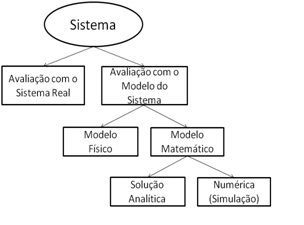
\includegraphics[width=\columnwidth]{./figures/011-Simulacao.jpg}
	\captionof{figure}{Simulação em Modelagem de Sistemas\cite{1}}
	\label{Figure-011-Simulacao}
}

O modelo matemático, por sua vez, pode ser definido como ``uma
representação, em termos matemáticos, do comportamento de objetos e dispositivos
reais''\cite{2} (tradução nossa). Esse modelo pode ser analítico ou de
simulação, que diferem pela natureza de suas soluções. Modelos analíticos
possuem como solução, uma equação fechada que descreve o comportamento do
sistema ao longo do tempo\cite{1}.

Modelos de simulação são solucionados por meio da execução de um programa que
gera amostras do comportamento do sistema, que permite realização de análises
do sistema\cite{1}. As etapas de desenvolvimento desse tipo de modelo é
descrita na figura \ref{Figure-012-EtapaSimulacao}.

O problema a ser tratado pela simulação é a análise comportamental da reação de
armadilhamento com desativação ao longo do tempo. Para uma formulação apropriada
deste problema e o posterior desenvolvimento de um modelo conceitual para tal
sistema, primeiro deve ser analisado o problema de forma mais simples, sem
desativação da armadilha, cujo modelo já possui solução analítica na
bibliografia. Esse modelo corresponde a uma versão discreta do modelo de
Smoluchowski\cite{5}.

{ \centering
	\hfill \break
	\captionsetup{type=figure}
	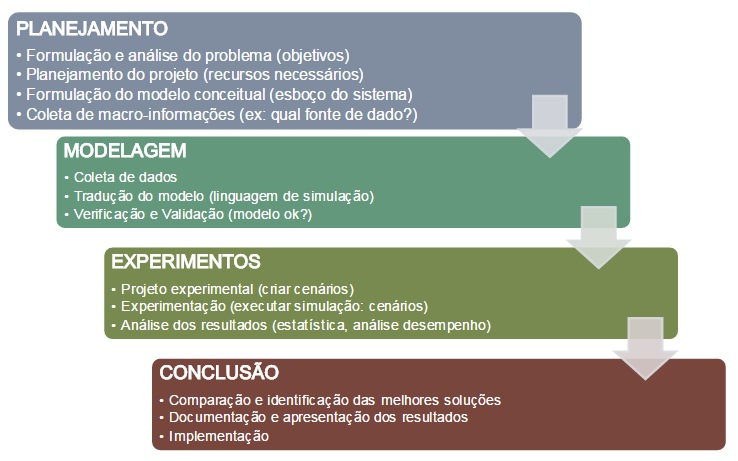
\includegraphics[width=\columnwidth]{./figures/012-EtapaSimulacao.jpg}
	\captionof{figure}{Etapas do processo de simulação\cite{1}}
	\label{Figure-012-EtapaSimulacao}
}


\section{Modelo de Smoluchowski}

\lettrine{S}{moluchowski} propôs uma modelagem do processo de armadilhamento a partir de uma
armadilha ou catalisador esférico de raio r, no qual as partículas reagem e saem
do sistema instantaneamente ao tocar a borda dessa esfera. Inicialmente, as
partículas estão distribuídas com concentração uniforme $\rho_0$ de partículas
ao redor da esfera\cite{3}. A variação da concentração dos reagentes em um
ponto x fora da esfera ao longo do tempo t, $\rho(x,t)$, é dada pela
equação\cite{3}:

{
\setlength{\belowdisplayskip}{0pt} \setlength{\belowdisplayshortskip}{0pt}
\setlength{\abovedisplayskip}{0pt} \setlength{\abovedisplayshortskip}{0pt}

\begin{equation}
  \frac{\partial}{\partial t}\rho(x,t) = D\nabla^2\rho(x,t), x>r,
  \label{Equation-021}
\end{equation}
}

\noindent sendo D o coeficiente de difusão dos reagentes. E já que os reagentes
que tocam a borda da esfera saem do sistema instantaneamente, a densidade de
partículas nessa região é 0, ou seja\cite{3}:

{
\setlength{\belowdisplayskip}{0pt} \setlength{\belowdisplayshortskip}{0pt}
\setlength{\abovedisplayskip}{0pt} \setlength{\abovedisplayshortskip}{0pt}

\begin{equation}
  \rho(x,t)|_{x=r} = 0
  \label{Equation-022}
\end{equation}
}

Tornando o problema discreto, pode-se considerar o sistema como uma rede de
sítios em que cada um desses sítios pode estar vazio, ocupado por um reagente
ou por um catalisador\cite{3}.  Dessa forma, definindo c como a concentração de
armadilhas na rede e S(t) o número de sítios ocupados por um reagente até o
tempo t, a probabilidade de sobrevivência Ps de sobrevivência de uma partícula
no instante t é\cite{6}:

{
\setlength{\belowdisplayskip}{0pt} \setlength{\belowdisplayshortskip}{0pt}
\setlength{\abovedisplayskip}{0pt} \setlength{\abovedisplayshortskip}{0pt}

\begin{equation}
  P_s(t) = \left<(1-c)^{S(t)}\right>
  \label{Equation-023-Probabilidade}
\end{equation}
}

A equação \ref{Equation-023-Probabilidade} é difícil de ser solucionada
analiticamente\cite{3}. Mas caso fosse solucionada, a densidade dos reagentes no
tempo t poderia ser obtida da seguinte forma:

{
\setlength{\belowdisplayskip}{0pt} \setlength{\belowdisplayshortskip}{0pt}
\setlength{\abovedisplayskip}{0pt} \setlength{\abovedisplayshortskip}{0pt}

\begin{equation}
  \rho(t) = \rho_0P_s(t)
  \label{Equation-024}
\end{equation}
}

Para tempos curtos, pode-se utilizar a seguinte aproximação para a equação
\ref{Equation-023-Probabilidade}:

{
\setlength{\belowdisplayskip}{0pt} \setlength{\belowdisplayshortskip}{0pt}
\setlength{\abovedisplayskip}{0pt} \setlength{\abovedisplayshortskip}{0pt}

\begin{equation}
  P_s(t) \approx (1-c)^{\left<S(t)\right>}
  \label{Equation-025}
\end{equation}
}

Para definir essa concentração em tempos longos, é feito uma outra simplificação
no modelo, tornando-o unidimensional. Dessa forma, existe um espaço L entre duas
armadilhas consecutivas no qual os reagentes podem circular livremente sem que
um sítio ocupe mais de um reagente. Para cada um desses espaços, sabe-se que a
concentração de reagentes nos sítios ocupados por armadilhas (0 e L) são sempre
0. Em um sítio intermediário x, a concentração inicial de reagente é $\rho_0$ e,
ao longo do tempo, essa concentração diminui com a seguinte taxa\cite{3}:

{
\setlength{\belowdisplayskip}{0pt} \setlength{\belowdisplayshortskip}{0pt}
\setlength{\abovedisplayskip}{0pt} \setlength{\abovedisplayshortskip}{0pt}

\begin{equation}
  \frac{\partial \rho}{\partial t} = D\frac{\partial^2 \rho}{\partial x^2}
  \label{Equation-026-TempoLongo}
\end{equation}
}

A equação \ref{Equation-026-TempoLongo} possui uma solução analítica aproximada,
como segue\cite{3}:

{
\setlength{\belowdisplayskip}{0pt} \setlength{\belowdisplayshortskip}{0pt}
\setlength{\abovedisplayskip}{0pt} \setlength{\abovedisplayshortskip}{0pt}

\begin{equation}
  \rho(t) \approx exp\left[ -\frac{3}{2} (2\pi^2c^2Dt)^{1/3} \right]
  \label{Equation-027-Decaimento}
\end{equation}
}


\section{Modelos com Desativação}

Abordaremos agora o modelo de reação-difusão com desativação de material
catalítico \cite{7}. O modelo trabalha sobre uma rede unidimensional de
sítios, onde cada sítio pode ser uma armadilha (um sítio catalítico) ou um sítio
inativo (material suporte).

Os sítios não se movem na rede durante a dinâmica e
as armadilhas (material catalítico) são distribuídas aleatoriamente com
recobrimento $\sigma_0$, enquanto os reagentes são distribuidos aleatoriamente
sobre os sítios inativos com recobrimento $\theta_0$. A distribuição de
reagentes e armadilhas respeita o vínculo $\sigma_0 + \theta_0 \leq 1$ e ela é
realizada antes de simularmos processo modelado. Não há fluxo de reagentes ou
reposição de armadilhas no decorrer da dinâmica.

A dinâmica do modelo se dá através da difusão de reagentes, que, ao se depararem
com um sítio ativo, reagem e saem instantaneamente do sistema, na forma de
produto.

O coeficiente de difusão é dado por $\mathcal{D}$, cujo valor expressa
o número de tentativas de se executar um passo do tamanho da rede, por unidade
de tempo, para cada reagente. A dinâmica de difusão respeita ainda o princípio
de volume excluído entre reagentes, de forma que um reagente tem execução de um
passo rejeitada quando a intenção do passo tem como alvo um sítio ocupado por
outro reagente.

Um reagente pode desativar o sítio ativo que ocupa com probabilidade \textit{p}
de modo que a dinâmica pode ser representada pelas equações:

{
\setlength{\belowdisplayskip}{0pt} \setlength{\belowdisplayshortskip}{0pt}
\setlength{\abovedisplayskip}{0pt} \setlength{\abovedisplayshortskip}{0pt}

\begin{equation}
  A + C \longrightarrow C \qquad c/ prob. 1 - p,
  \label{Equation-031-ModeloTradicional}
\end{equation}
\begin{equation}
  A + C \longrightarrow 0 \qquad c/ prob. p,
  \label{Equation-032-ModeloEnvenenamento}
\end{equation}
}

\noindent onde \textit{A} representa o reagente que difunde, \textit{C}
representa uma armadilha e 0 representa um sítio inativo.

A equação \ref{Equation-031-ModeloTradicional} corresponde ao modelo de armadilhamento, pois
os reagentes ficam confinados entre dois sítios catalíticos; enquanto a equação
\ref{Equation-032-ModeloEnvenenamento} é chamada de reação de envenenamento (ou
\textit{poisoning}), pois existe desativação de sítio catalíticos. O modelo está
representado graficamente na figura \ref{Figure-031-EsquemaModelo}.

Da forma como foi concebido, é natural concluir que existirão duas fases
distintas para tempos longos: uma em que o número de reagentes decai até zero
(que ocorre com baixa probabilidade de desativação e baixa concentração de
reagentes); outra em que um número finito de reagentes sobrevive após a
desativação de todos os sítios catalíticos do sistema (que ocorre com alta
probabilidade de desativação e alta concetração de reagentes). O sistema se
comporta segundo dinâmica de uma reação bimolecular de aniquilação na fronteira
entre essas duas fases,

{
\setlength{\belowdisplayskip}{0pt} \setlength{\belowdisplayshortskip}{0pt}
\setlength{\abovedisplayskip}{0pt} \setlength{\abovedisplayshortskip}{0pt}

\begin{equation}
  A + B \longrightarrow 0,
  \label{Equation-032-ModeloBimolecular}
\end{equation}
}

\noindent onde sítios catalíticos desempenham papel da segunda espécie reativa
\textit{B}.

{
  \centering
  \captionsetup{type=figure}
	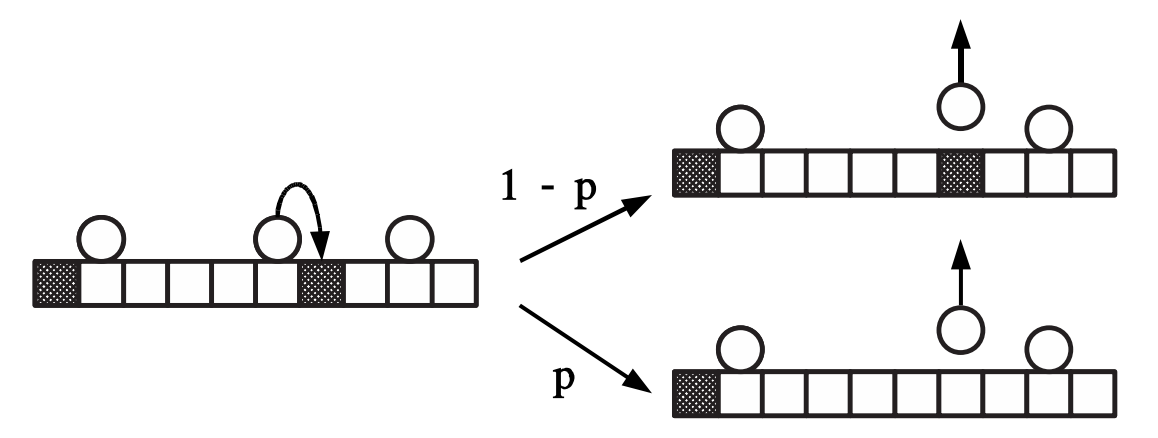
\includegraphics[width=\columnwidth]{./figures/031-EsquemaModelo.png}
  \captionof{figure}{Representação esquemática da dinâmica do modelo.
    Os sítios catalíticos (armadilhas) estão representados por quadrados pretos,
    enquanto sítios inativos, por quadrados brancos. Os círculos representam
    reagentes que difundem pela rede. Quando um reagente se desloca para uma
    armadilha, deixa o sistema instantaneamente. Quando este evento ocorre, com
    probabilidade \textit{p}, o sítio perde sua atividade catalítica e passa a
    ser um sítio inativo (\ref{Equation-032-ModeloEnvenenamento}). Com probabilidade 1 -
    \textit{p}, o sítio matém sua condição de sítio catalítico
    (\ref{Equation-031-ModeloTradicional}) \cite{3}.}
	\label{Figure-031-EsquemaModelo}
}


\section{Metodologia}

Para a execução da simulação, um primeiro passo é definir aspectos do ambiente
simulacional.

A implementação da rede unidimensional do se sistema se dá por um arranjo, onde
cada posição do arranjo pode: conter um sítio inativo desocupado; conter um
sítio inativo ocupado por um reagente; conter um sítio ativo.

Três listas encadeadas são utilizadas como estruturas auxiliares para
distribuir uniformemente os sítios ativos e os reagentes na rede. Um sítio
aleatoriamente escolhido é removido de uma primeira lista auxiliar, de forma a
garantir que um sítio não seja escolhido duas vezes, enquanto uma segunda lista
auxiliar mantém referência para todos os sítios da rede. Uma terceira lista
armazena a sequência de posições dos sítios aleatóriamente escolhidos para
reagentes, com finalidade de facilitar a simulação do processo de difusão. A
lista encadeada auxiliar que mantém referência de todos os sítios da rede é
mapeada em um arranjo linear após distribuição aleatória de sítios catalíticos e
reagentes.

São parâmetros de simulação: número de execuções independentes de cada dinâmica
$M$; duração da dinâmica $Z$, em termos do número de tentativas de se executar
um passo, onde cada reagente do sistema tenta executar $Z$ passos; o tamanho da
rede $N$, correspondente ao número de sítios contidos por ela; e coeficiente de
difusão $\mathcal{D}$, correspondente ao número de tentativas de se executar um
passo do tamanho da unidade da rede, por unidade de tempo, por reagente.

O gerador de números pseudo-aleatórios utilizado nas simulações é o algoritmo
\texttt{Ranq1} \cite{8}. Cada número pseudo-aleatório gerado depende do número
gerado anteriormente, sendo que o primeiro elemento depende do valor fornecido
como semente ao algoritmo. Essa característica é determinante para que todas as
$M$ execuções independentes aconteçam sequencialmente, sem que um i-ésimo valor
pseudo-aleatório gerado seja considerado mais de uma vez ou desconsiderado.

A difusão de reagentes respeita o princípio de volume excluído, de forma que se
determinado reagente tenta executar passo com destino a um sítio previamente
ocupado, tal tentativa é rejeitada e o reagente não se desloca nessa iteração.
Os resultados da simulação são: o número de passos executados por cada reagente
e a dupla composta pela contagem de reagentes e pela contagem de sítios
catalíticos, por iteração da rede e por execução independente, correspondentes a
um total de $M \times Z$ duplas.

Os valores dos parâmetros utilizados na simulação foram: $N = 2^{20}$,
$\mathcal{D} = 1$, $Z = 10^8$.


\section{Resultados}

\lettrine{P}{rimeiramente}, foram realizadas simulações para o caso em que a probabilidade p
de envenenamento é muito baixa. No caso extremo, essa probabilidade é 0 e o
sistema se comporta de acordo com a equação \ref{Equation-027-Decaimento}, para
sistemas sem envenenamento. Mas como mostrado pela figura
\ref{Figure-052-Resultado}, essa equação descreve bem sistemas com p pequenos.
Nesses sistemas, em que $\sigma_0 >> p*\theta_0$, é possível perceber pela
figura que a quantidade de reagentes decaem em uma lei de potência e tendem a
acabar com o passar do tempo. Esse comportamento é esperado já que o
envenenamento ocorre com pouca frequência no sistema com esse tipo de regime,
então a chance dos regentes reagirem e saírem do sistema é grande. Por isso, o
sistema tende a perder poucos catalisadores e perder todos os reagentes.

{
	\captionsetup{type=figure}
	\hfill \break
	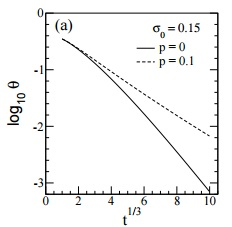
\includegraphics[width=\columnwidth]{./figures/052-Resultado.jpg}
	\captionof{figure}{Comportamento dos reagentes com o tempo para regimes em que
		os regentes tendem a se extinguir}
	\label{Figure-052-Resultado}
}

Posteriormente, foram realizadas simulações para o caso em que o sistema possui
probabilidade de envenenamento p alta e concentração inicial de reagentes
$\theta_0$ também alta ao passo que a concentração inicial de catalisadores
$\sigma_0$ se manteve constante. Sistemas com esse regime apresentam um
decaimento de reagentes muito grande no início, já que a concentração deles
é grande, mas com o passar do tempo esse decaimento vai ocorrendo de forma
cada vez mais lenta até que não haja mais nenhum decaimento, como pode ser
observado na figura \ref{Figure-053-Resultado}. Isso ocorre porque a chance de
ocorrer envenenamento é grande, o que faz com que o decaimento do número de
reagentes também seja grande e, no fim, todos os catalisadores são desativados e
os reagentes restantes permanecem no sistema.

{ \centering
	\captionsetup{type=figure}
	\hfill \break
	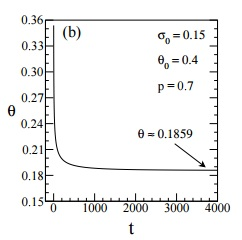
\includegraphics[width=\columnwidth]{./figures/053-Resultado.jpg}
	\captionof{figure}{Comportamento dos reagentes com o tempo para regimes em que
	 	os catalisadores tendem a se extinguir}
	\label{Figure-053-Resultado}
}

Também foram simulados sistemas de reação-difusão com envenenamento na
criticalidade, ou seja, sistemas nos quais $\sigma_0 = p*\theta_0$. Como
esperado, percebe-se na figura \ref{Figure-051-Resultado} um decaimento em lei
de potência do número de reagentes no tempo para esses sistemas e, além disso,
as curvas em uma escala log-log apresentam uma reta com inclinação de,
aproximadamente, $-1/4$, como prevê a equação REFERENCIAR!!.

{ \centering
	\captionsetup{type=figure}
	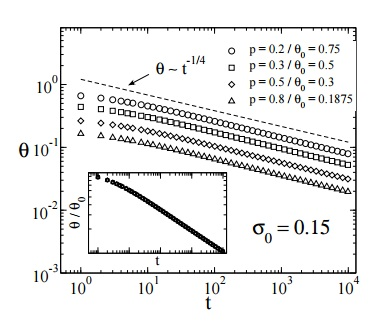
\includegraphics[width=\columnwidth]{./figures/051-Resultado.jpg}
	\captionof{figure}{Comportamento dos reagentes no tempo em um sistema de
		reação-difusão na criticalidade. No inset observa-se todas as curvas
		colapsadas}
	\label{Figure-051-Resultado}
}

As simulações já apresentadas descrevem sistemas com envenenamento longe da
criticalidade e exatamente na criticalidade. As últimas simulações descrevem
sistemas próximos da criticalidade, com regimes em que os reagentes tendem a
acabar ($\sigma_0 > p*\theta_0$). A figura \ref{Figure-054-Resultado} descreve
esses sistemas próximos da criticalidade e, como pode-se perceber, no início os
reagentes decaem de acordo com a lei de potência prevista para sistemas na
criticalidade (o início dos sistemas no primeiro gráfico apresenta comportamento
semelhante ao observado na figura \ref{Figure-051-Resultado}), mas em tempos
longos, o sistema se comporta como aquele da figura \ref{Figure-052-Resultado}.
A semelhança pode ser notada comparando o segundo gráfico da figura
\ref{Figure-054-Resultado} com a figura \ref{Figure-052-Resultado}.

{ \centering
	\captionsetup{type=figure}
	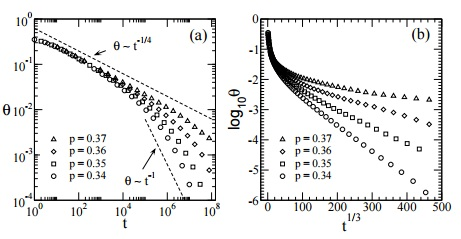
\includegraphics[width=\columnwidth]{./figures/054-Resultado.jpg}
	\captionof{figure}{Comportamento dos reagentes no tempo em sistemas de
		reação-difusão próximos da criticalidade}
	\label{Figure-054-Resultado}
}


\printbibliography

\end{multicols*}
\end{document}
